% Jig vision report: method comparison in the robot-cell simulator + procedure for the real TM5-900.
% The long text version (kept; the short picture report is jig_vision_report.tex)
% Build: latexmk -pdf jig_vision_report_detailed.tex   (figures: python make_figures.py)
\documentclass[11pt,a4paper]{article}

\usepackage[utf8]{inputenc}
\usepackage[T1]{fontenc}
\usepackage[margin=22mm]{geometry}
\usepackage{amsmath,amssymb}
\usepackage{graphicx}
\usepackage{booktabs}
\usepackage{array}
\usepackage[table,dvipsnames]{xcolor}
\usepackage{listings}
\usepackage[font=small,labelfont=bf]{caption}
\usepackage{subcaption}
\usepackage{hyperref}
\usepackage{fancyhdr}
\usepackage{enumitem}
\usepackage{tcolorbox}

\definecolor{hdrblue}{HTML}{2F6FB5}
\definecolor{rowlt}{HTML}{EFF3F8}
\definecolor{codebg}{HTML}{F7F7F9}
\definecolor{good}{HTML}{3F7D58}

\hypersetup{colorlinks=true,linkcolor=hdrblue,urlcolor=hdrblue}
\pagestyle{fancy}
\fancyhf{}
\fancyhead[L]{\small MMA4002 DAM -- Robot cell: finding the jigs with a camera}
\fancyhead[R]{\small\thepage}
\renewcommand{\headrulewidth}{0.4pt}
\setlist{itemsep=1pt,topsep=3pt}

\lstset{basicstyle=\ttfamily\scriptsize,backgroundcolor=\color{codebg},frame=single,rulecolor=\color{gray!40},
  breaklines=true,columns=fullflexible,showstringspaces=false}
\newcommand{\hdr}[1]{\textcolor{white}{\textbf{#1}}}
\newcommand{\code}[1]{\texttt{\small #1}}

% numbers from the calibration test (tests/vision_lab/calibrate_test.py), filled in from its report.json
% generated by calib_numbers.py from calib_20261113-024202
\newcommand{\calibRun}{calib_20261113-024202}
\newcommand{\calibLayouts}{5}
\newcommand{\calibRms}{0.047}
\newcommand{\calibFx}{0.04}
\newcommand{\calibHePos}{0.15}
\newcommand{\calibHeRot}{0.08}
\newcommand{\calibFixPos}{2.34}
\newcommand{\calibFixRot}{0.41}
\newcommand{\calibFixTable}{1.84}
\newcommand{\calibHeTable}{0.97}
\newcommand{\calibHeFound}{0.02, 74.94, 52.86}
\newcommand{\calibCx}{1.3}
\newcommand{\calibFound}{24/25}
\newcommand{\calibMed}{0.03}
\newcommand{\calibMax}{1.20}
\newcommand{\calibFarMed}{0.07}
\newcommand{\calibFarMax}{0.96}
\newcommand{\calibRzMax}{0.31}


\title{\vspace{-14mm}\textbf{Finding the jigs with a camera}\\[1.5mm]
\large Three vision methods compared in the robot-cell simulator, and the procedure for the real TM5-900}
\author{Bjørge \quad (MMA4002 DAM, robot cell)}
\date{\today}

\begin{document}
\maketitle
\sloppy
\thispagestyle{fancy}
\vspace{-6mm}

\begin{tcolorbox}[colback=rowlt,colframe=hdrblue,title=\textbf{Outcome},fonttitle=\small,boxsep=1mm]
\small
\textbf{Use ArUco markers.} In 10 random jig layouts in the simulator, the marker method found every jig whose marker was
visible (40/40) with a median error of \textbf{0.14\,mm} and \textbf{0.07\,°}, never worse than \textbf{0.5\,mm / 0.4\,°},
from two different camera poses, and unchanged in darker, noisy or shadowed photos. It takes 0.2--0.4\,s per photo.
Colour matching was 3--10$\times$ less accurate (worst 4.3\,mm) and confuses the two touching blue bases; feature matching
(SIFT, as TMflow's pattern matching) made gross errors from an oblique view (up to 232\,mm).
The \textbf{plank rack} is the one hard jig: the standing planks hide any marker on it from the overview pose --
a second photo straight above the rack finds it (4 of 5 layouts, $\le$0.8\,mm).
The real-robot tools (calibration, capture, set-up) were run end to end in the simulator with known answers
(Section~\ref{sec:real}) and are ready for the lab, with the TM5's own camera or a USB webcam.
\end{tcolorbox}

\section{Goal and set-up}
\textbf{Goal.} Before a run, the robot must know where each jig really stands. The program was taught with the jigs in one
layout; when a jig is put back a few millimetres or degrees off, every taught point on it must move by the same amount.
A camera photo should give that move per jig: a shift $(x, y)$ in the robot base (mm) and a turn $r_z$ (deg), as a
$4\times4$ matrix $T_\text{move}$ with $p_\text{now} = T_\text{move}\,p_\text{taught}$ for any point of the jig.

\textbf{Simulator.} The tests ran in the group's own robot-cell simulator (cell v9: TM5-900, T-slot plate, bases A and B,
plank rack, the two guide halves, planks and frames). New for this work:
\begin{itemize}
\item a \textbf{tool camera} at the lens of the TM5's end module (taken from Techman's link-6 mesh: 75\,mm off the flange
axis, looking along the tool), $1280\times960$\,px, 45\,° vertical field of view, ideal pinhole;
\item each photo is saved with its camera matrix $K$, the camera pose $T_\text{base,cam}$ and the \textbf{true} pose of every
jig, plus (for reference photos) a position pass: the 3D point and object of every pixel;
\item ArUco markers (4$\times$4, 22\,mm) on a flat spot of each jig, placed automatically; a jig mover and a headless
renderer, so scripts can set layouts and take photos without anyone at the screen.
\end{itemize}
Everything is in \code{tests/vision\_lab/} and \code{tests/robot\_sim/} (see \code{OWN\_TOOL.md}).

\section{The three methods}
All three take a photo with its $K$ and $T_\text{base,cam}$ and return the same output: $(x, y, r_z)$ per jig.
\begin{description}[leftmargin=0pt,labelsep=4pt]
\item[ArUco markers.] The marker's four corners are found to sub-pixel precision, each corner's camera ray is cut with
the marker's known height, and a 2D rigid fit to the marker's taught corners gives the move. Needs a marker per jig and
its height; no reference photo.
\item[Colour.] The jig's colour (hue and saturation, learned from a reference photo of the taught layout) is segmented
inside a search area around the taught place, the blob is put on the jig's top height, and the reference blob is turned
($\pm$25\,°, coarse to fine) and shifted (phase correlation) onto it; the best overlap gives the move. No markers.
\item[Features (SIFT + PnP).] SIFT keypoints of the reference photo carry their true 3D point from the position pass;
they are matched in the new photo and \code{solvePnPRansac} gives the jig's full pose. This is the closest to TMflow's
calibrated pattern matching, and works from another camera pose. No markers.
\end{description}

\section{Test design}
Ten random layouts (seed 7): Base A, Base B and the plank rack each moved by up to $\pm$30\,mm and turned up to $\pm$10\,°;
the guide halves sit in Base B and moved with it, the parts on a base with that base. Each layout was photographed from
two poses -- \emph{top} (520\,mm above the middle of the jigs, looking down) and \emph{side} (another place, wrist turned
30\,°) -- with markers on and off. The top photos were also disturbed as in a lab: darker ($\times$0.55), noise + blur,
and a soft shadow band. References for colour and features were taken from the top pose. The error is the distance between
found and true pivot position, and the turn difference; 5 jigs $\times$ 10 layouts = 50 tries per case.

\section{Results}
\begin{table}[h]
\centering\small
\rowcolors{2}{rowlt}{white}
\begin{tabular}{l l c c c c c r}
\toprule
\rowcolor{hdrblue}
\hdr{Method} & \hdr{Photo} & \hdr{Found} & \hdr{Median mm} & \hdr{90\,\% mm} & \hdr{Worst mm} & \hdr{Worst °} & \hdr{Time} \\
\midrule
\textbf{ArUco} & top, markers & 40/50 & \textbf{0.14} & 0.21 & \textbf{0.44} & 0.26 & 0.4\,s \\
\textbf{ArUco} & side, markers & 40/50 & 0.34 & 0.44 & 0.49 & 0.37 & 0.2\,s \\
Colour & top & 40/50 & 0.49 & 1.49 & 2.93 & 6.50 & 21\,s \\
Colour & side & 40/50 & 0.94 & 3.59 & 4.33 & 2.55 & 19\,s \\
Features & top & 40/50 & 0.64 & 1.73 & 8.51 & 0.90 & 5.8\,s \\
Features & side & 32/50 & 2.62 & 7.75 & 231.8 & 171.9 & 6.0\,s \\
\bottomrule
\end{tabular}
\caption{Clean photos, 10 layouts. ``Found'' counts all five jigs; all methods except features miss only the plank rack
(10/50). Times on the laptop, not optimised for colour and features.}
\label{tab:main}
\end{table}

\begin{figure}[h]
\centering
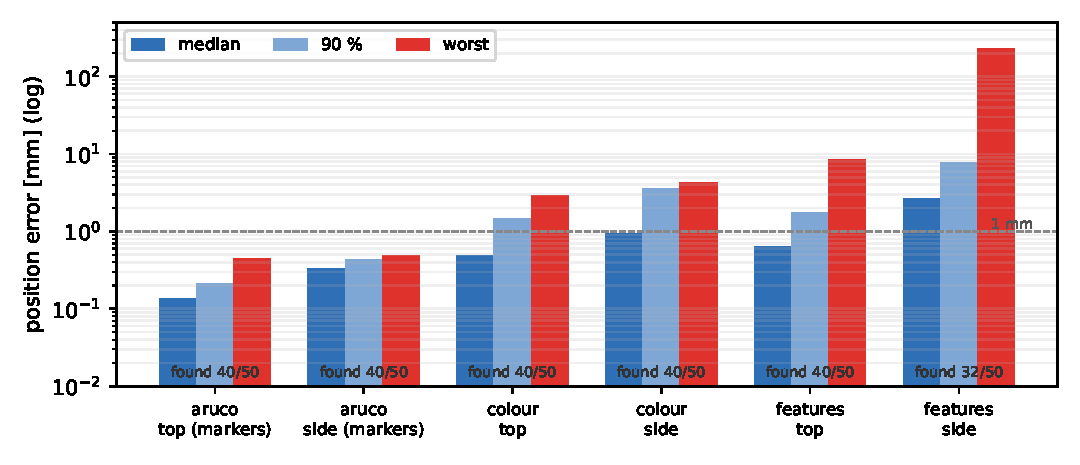
\includegraphics[width=0.92\linewidth]{figures/errors.pdf}
\vspace{-2mm}
\caption{Position error per method and camera pose (log scale): median, 90\,\% and worst. Only ArUco stays below 1\,mm
in every case.}
\label{fig:errors}
\end{figure}

\textbf{ArUco} is the most accurate, the most repeatable and the fastest, and it is the only method that never failed
gross for a jig it reported. It is also insensitive to the lab-like disturbances (Fig.~\ref{fig:dist}): the median stays
at 0.12--0.14\,mm and the worst at 0.43--0.45\,mm, because a printed black/white square keeps its corners in the dark, in
noise and under a shadow. From the oblique side pose the median doubles (0.34\,mm) but the worst case stays under 0.5\,mm.

\textbf{Colour} is good on the guides (median 0.3--0.5\,mm) but 24 of its 25 errors above 2\,mm are on the two bases:
they are the same blue and touch, so their blobs merge in the search area. It cannot see the grey rack at all (grey is
everywhere in the cell), and it depends on the learned colours staying the same under the lab light.

\textbf{Features} need no markers and see the rack sometimes (4/10, $\approx$4\,mm), but they are least reliable: from
the side pose 14 of 73 results were more than 5\,mm off, up to 232\,mm and 172\,° -- PnP on a few wrong matches gives a
confident but wrong pose (Fig.~\ref{fig:overlays}, right). In a real cell with shiny 3D-printed parts this gets worse.

\begin{figure}[h]
\centering
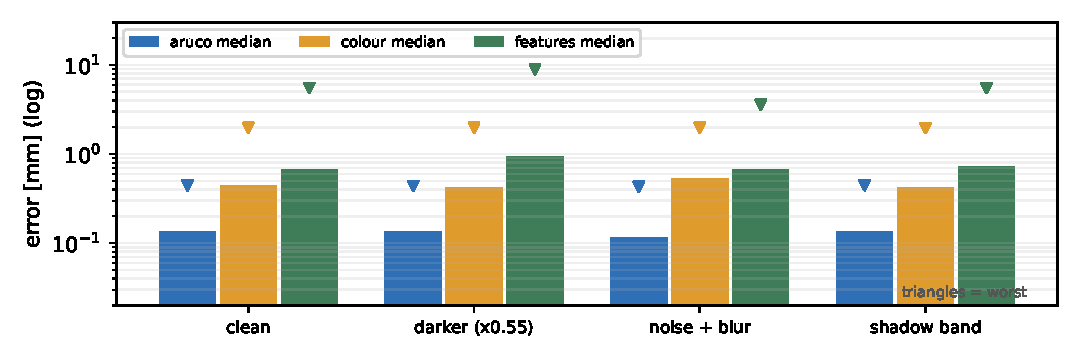
\includegraphics[width=0.92\linewidth]{figures/disturbances.pdf}
\vspace{-2mm}
\caption{Top pose with markers, under lab-like disturbances: median (bars) and worst (triangles) position error.}
\label{fig:dist}
\end{figure}

\begin{figure}[h]
\centering
\begin{subfigure}{0.49\linewidth}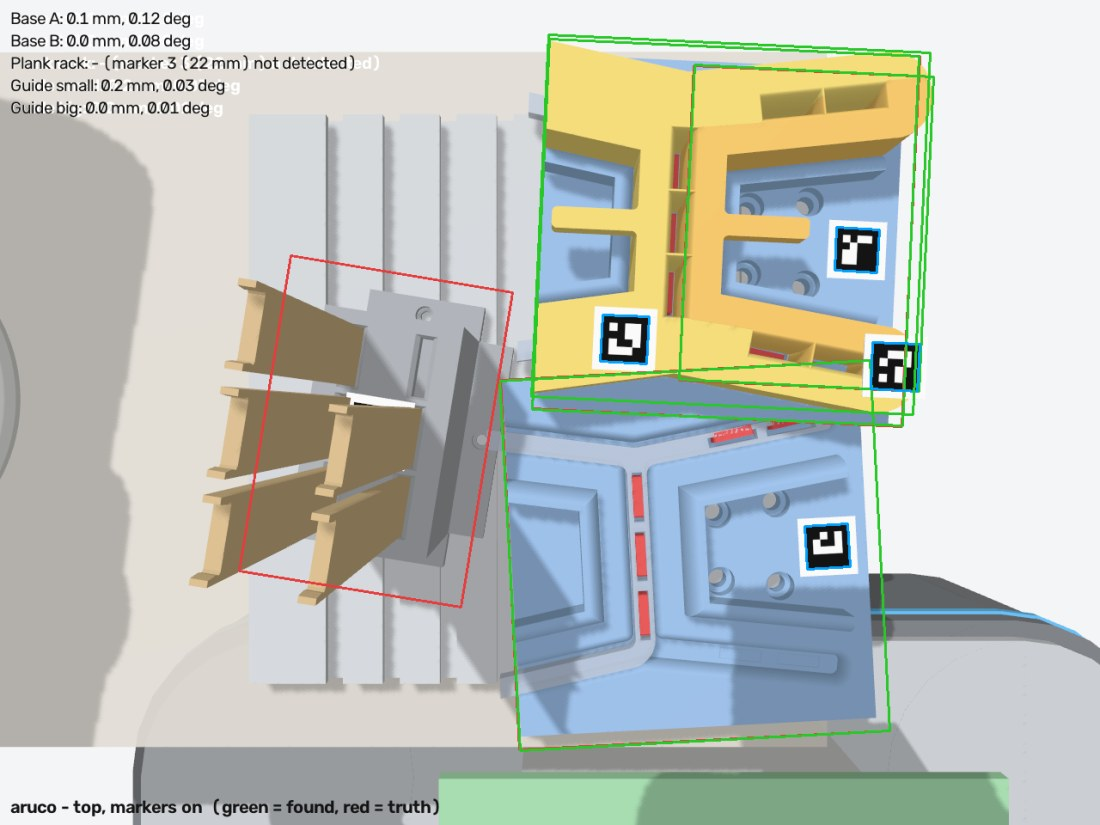
\includegraphics[width=\linewidth]{figures/aruco_top.jpg}\caption{ArUco, top pose: every
outline on its truth; the rack's marker is hidden by the planks.}\end{subfigure}\hfill
\begin{subfigure}{0.49\linewidth}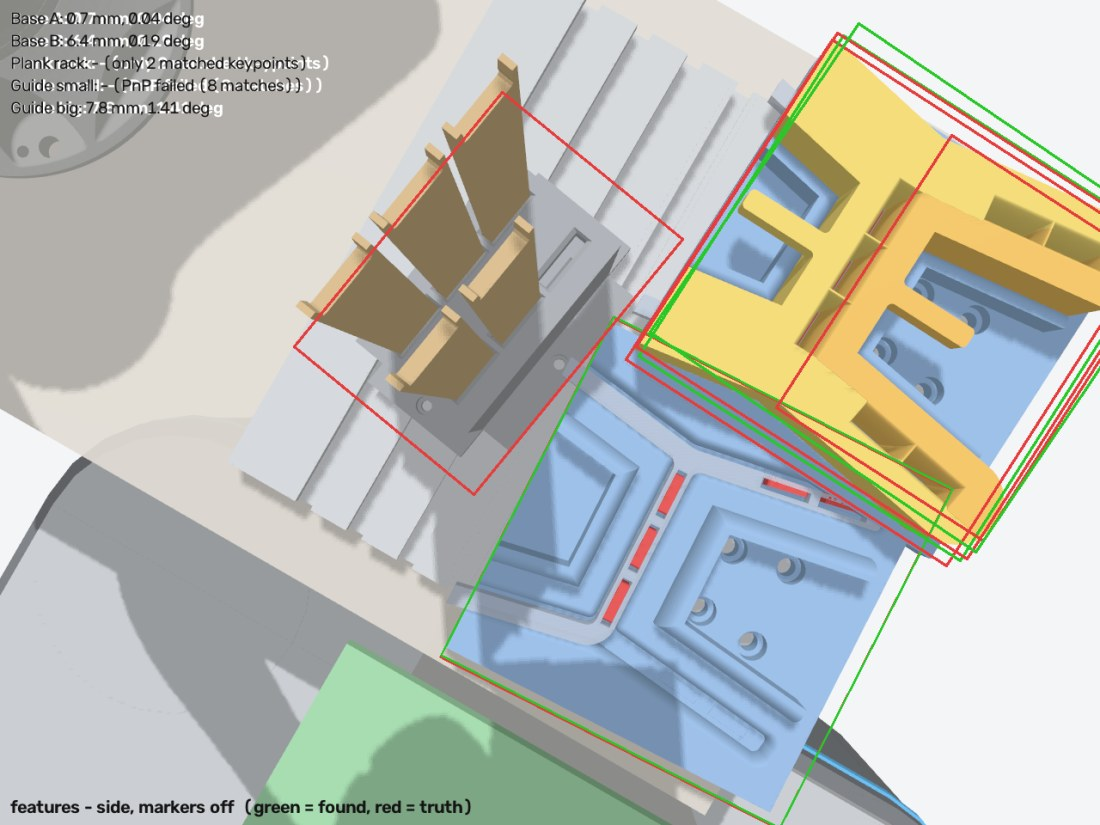
\includegraphics[width=\linewidth]{figures/features_side.jpg}\caption{Features, side pose:
Base B and the big guide 6--8\,mm off, rack and small guide lost.}\end{subfigure}
\caption{What the methods found (green) against the truth (red), layout 1.}
\label{fig:overlays}
\end{figure}

\textbf{The plank rack.} No flat spot on the rack is clear of the standing planks, so a marker on it is hidden from the
overview pose (0/50). Two remedies were tried: a marker lifted on a post above the planks (would need $\approx$160\,mm:
not practical) and \textbf{a second photo straight above the rack}. With the camera above it, ArUco found the rack in
4 of 5 layouts with errors of 0.03--0.8\,mm (5 layouts, seed 11; the other jigs 0.05--0.35\,mm in the same run). With a
camera on the tool this costs one extra robot move; \code{jig\_vision.py} takes several photos and uses, per jig, the one
where its marker is nearest the image centre (Fig.~\ref{fig:rack}).

\begin{figure}[h]
\centering
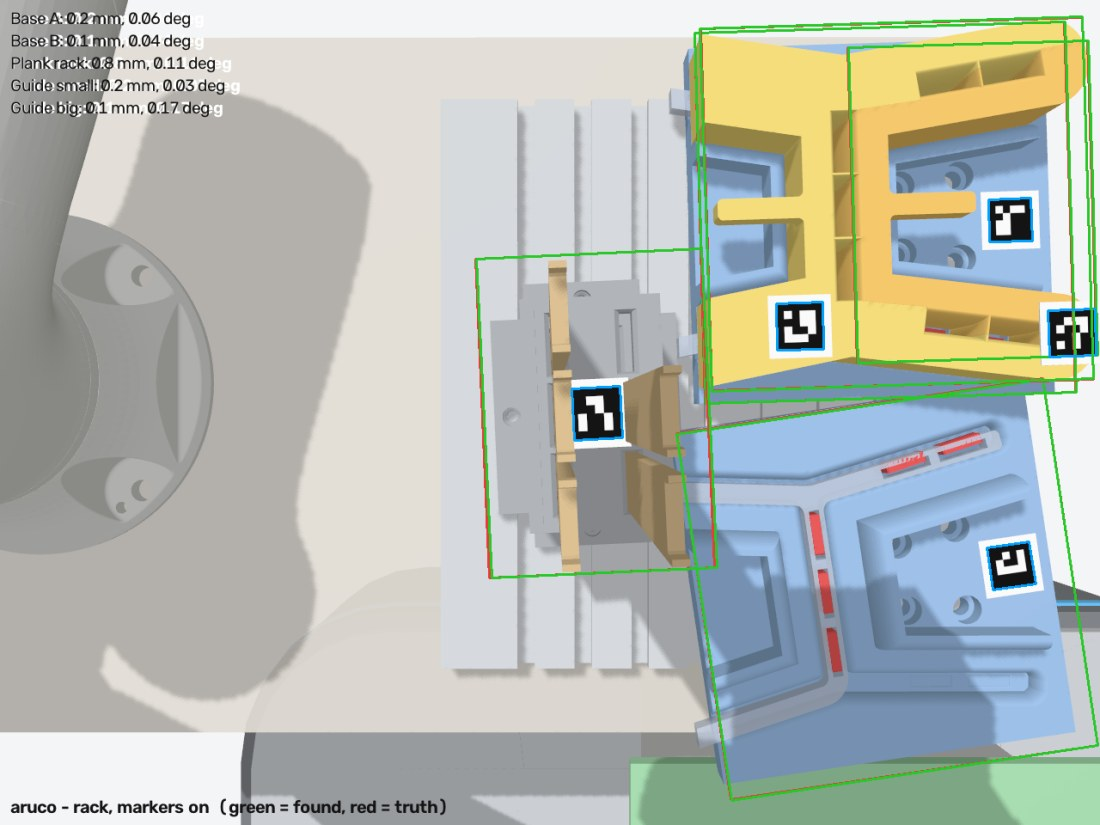
\includegraphics[width=0.62\linewidth]{figures/aruco_rack.jpg}
\caption{ArUco from straight above the rack: its marker (left of centre, on the grey rack) is now visible past the
planks and the rack is found (green on red).}
\label{fig:rack}
\end{figure}

\section{Ready for the real robot}\label{sec:real}
\textbf{Camera:} first choice is the TM5's own eye-in-hand camera -- the simulator's camera sits at its lens. TMflow's
\emph{External Detection} vision step sends the image over HTTP to the laptop (\code{tm\_camera.py}); this route is
taken from Techman's ROS driver and not yet tried on our robot (TMflow version). If it is missing, a \textbf{USB webcam}
on the tool or above the table does the same job (\code{real\_capture.py}).
Five scripts make the real photos look exactly like the simulator's, so \code{jig\_vision.py} runs unchanged:
\begin{description}[leftmargin=0pt,labelsep=4pt]
\item[\code{print\_markers.py}] A4 sheets at 1:1 with a 100\,mm check bar: jig markers (ids 1--5 = Base A, Base B, rack,
small guide, big guide; 30\,mm) and a ChArUco calibration board (7$\times$5 squares of 30\,mm).
\item[\code{calibrate.py}] lens calibration from 10--20 board photos; then either \emph{hand-eye} (camera on the tool:
the robot looks at the still board from 10--15 poses) or \emph{fixed} (one photo + three board points touched with the
robot tip).
\item[\code{real\_capture.py}] webcam frame + robot pose (Modbus, read only -- it never moves the robot) $\rightarrow$
undistorted photo + JSON; \code{live} shows the camera with the markers it sees.
\item[\code{tm\_camera.py}] the same for the TM camera: an HTTP server that saves every image TMflow sends, with the
pose, and logs each request (tested in the simulator: output identical to \code{real\_capture.py}).
\item[\code{real\_setup.py}] records where each marker is in the taught layout; later photos are measured against it.
\end{description}

\textbf{Tested end to end in the simulator} (\code{calibrate\_test.py}, known answers): 15 board photos from different
wrist poses, then the full jig procedure with the calibrated camera on \calibLayouts{} new layouts.
\begin{table}[h]
\centering\small
\rowcolors{2}{rowlt}{white}
\begin{tabular}{>{\raggedright}p{48mm} >{\raggedright}p{58mm} >{\raggedright\arraybackslash}p{44mm}}
\toprule
\rowcolor{hdrblue}
\hdr{Step} & \hdr{Result} & \hdr{True value / meaning} \\
\midrule
Lens (intrinsics) & RMS \calibRms\,px; $f$ \calibFx\,\%, centre \calibCx\,px off & sim camera: ideal pinhole \\
Camera on the tool (hand-eye) & found (\calibHeFound)\,mm: \calibHePos\,mm, \calibHeRot\,° off & true (0, 75, 53)\,mm (TM5 mesh) \\
\quad what that does on the table & \calibHeTable\,mm (worst over the image) & a table point seen through it \\
Fixed camera (touch 3 points, 0.3\,mm noise) & \calibFixPos\,mm, \calibFixRot\,° off; table \calibFixTable\,mm & camera pose; on the table \\
Jigs with the calibrated camera & found \calibFound; median \calibMed\,mm, worst \calibMax\,mm & at the marker \\
\quad same, 100\,mm away (a grip point) & median \calibFarMed\,mm, worst \calibFarMax\,mm; worst \calibRzMax\,° & what the gripper sees \\
\bottomrule
\end{tabular}
\caption{The real-robot procedure run in the simulator. The webcam's real lens and print quality are the only parts
the simulator cannot test.}
\label{tab:calib}
\end{table}
Hand-eye found the camera on the tool to 0.15\,mm and 0.08\,°. Seen on the table, that is up to \calibHeTable\,mm at the
image edge -- yet the jigs came out at a median of \calibMed\,mm. The reason matters for the lab: every jig is measured
\emph{against the taught-layout photo, taken with the same camera}, so most calibration error is the same in both photos
and cancels. The fixed camera with three touched points is the weaker option (\calibFixTable\,mm on the table with
0.3\,mm touch noise); it cancels too, as long as the camera is never bumped. Touch points far apart (the board's corners)
and, if possible, prefer the camera on the tool. The two rack results near 1\,mm come from its marker seen at a slant
past the planks.

\section{Procedure for the lab (next week)}
\textbf{First:} in a TMflow vision job on the eye-in-hand camera, look for \emph{External Detection}; point it at
\code{http://<laptop IP>:6189}, run \code{tm\_camera.py calib}, and check \code{tm\_camera.log} shows a saved image
(allow Python through the Windows firewall). Then use \code{tm\_camera.py calib|photo} wherever the steps below say
\code{real\_capture.py}. \textbf{Bring:} as fallback a USB webcam (1080p, manual focus) with a mount, the printed sheets (check the 100\,mm bar), the board glued on a stiff flat plate, the laptop with the repo.
The scripts only \emph{read} the robot; all moves are done by hand-jogging in TMflow at low speed, from above.
\begin{enumerate}
\item \code{python tests/vision\_lab/print\_markers.py} -- print at 100\,\%; glue markers on the jigs (rack: on its top,
it is read from above; small guide: on a tab). Measure each marker's height with the TCP tip.
\item \textbf{Lens:} \code{real\_capture.py live} to see the view; then 15$\times$ \code{real\_capture.py calib} with the
board tilted, in all parts of the image; \code{calibrate.py intrinsics tests/vision\_lab/calib\_shots} (RMS should be
$<$0.5\,px).
\item \textbf{Where the camera is:} on the tool -- board flat and \emph{still}, jog to 10--15 poses (tilt 10--25\,° each
way, turn the wrist), \code{real\_capture.py calib -{}-out tests/vision\_lab/he\_shots} at each (a folder of its own:
the lens photos had a moving board), then \code{calibrate.py handeye tests/vision\_lab/he\_shots} (check: ``agrees
within'' a few mm); fixed -- one \code{calib} photo, touch O, +x, +y far apart on the board, \code{calibrate.py fixed}.
\item \textbf{Taught layout:} jigs where the program was taught; \code{real\_capture.py photo} from the overview pose and
from straight above the rack; \code{real\_setup.py <both photos> -{}-size 30 -{}-z "Base A=..." ...}.
\item \textbf{Check:} move one jig by a known amount (e.g. 10\,mm along a T-slot), photograph, run
\code{jig\_vision.py <photos> -{}-methods aruco -{}-save moves.json}: the reported move must match within
$\approx$1\,mm.
Then the taught points: $p_\text{now}=T_\text{move}\,p_\text{taught}$ (\code{jig\_vision.move\_point}).
\end{enumerate}

\section{Limits and next steps}
\begin{itemize}
\item The simulator's camera is ideal and its light even; a real camera adds lens distortion (calibrated away), blur
and glare on the PLA. Expect real errors a few times larger than here -- still well under the grip tolerance if they
stay near 1\,mm. Step 5 above is the real test.
\item Marker heights must be measured: a 1\,mm height error moves the result by up to $\approx$0.4\,mm at the image edge.
\item Only plane moves (x, y, $r_z$) are measured; a jig that is tilted or lifted is not detected.
\item Not built yet: applying $T_\text{move}$ to the taught points in the replay script (\code{v4\_replay.py}) -- the
next step once step 5 passes. Colour and features are kept in the code for comparison, but are not recommended.
\end{itemize}

\end{document}
